\section{Assessing predictive performance}
\label{sec:prediction_model_comparison}


To compare the four prediction methods, we implemented the first two in the \textsf{transitr} application and, using a single day of data, run the program, storing all arrival time estimates, the uncertainty, as well as the 5\% and 90\% quantiles\footnote{Initially we used a symmetric 95\% prediction interval, but this was often highly skewed by a few very late particles.}. The actual (reported) arrival times are then used to compare the accuracy of each method. For the historical data, we compare the mean with the actual arrival time. For the schedule-delay method, the arrival time for all upcoming stops was predicted after each new observation, and the prediction error computed.

\begin{itemize}
\item yes, rewrite the above para to make more sense please.
\item and, the below might need some more words about MAE/MAPE \ldots
\end{itemize}

We used \gls{rmse}, \gls{mae}, and \gls{mape} as comparison criteria (see \cref{app:error-functions}).
\Gls{rmse} is the mean squared difference (in seconds) between the predicted and actual arrival times. Of course, since predictions change over time, we also compute \gls{rmse} by \emph{time until (actual) arrival}, allowing us to compare the models at different time points, as well as by stop sequence and time of day.


Another criteria we are interested in is the \gls{picp}, which is only available for the three methods for which we can construct an 85\% \gls{ppi}: for the particle filter, this is achieved by sorting the particles in order of arrival time, and then taking the $\lfloor q_\text{lower} N^\star\rfloor^{\text{th}}$ particle as the lower bound, and the $\lceil q_{\text{upper}} N^\star\rceil^{\text{th}}$ particle as the upper bound (more details in \cref{app:particle_summaries}). For the 85\% interval, we used $q_\text{lower} = 0.05$ and $q_\text{upper} = 0.9$. For the normal approximation and historical arrival methods, the inverse \gls{cdf} provides the required quantiles. The results are displayed in \cref{tab:model_results_rmse} and \cref{fig:model_results_rmse_time,fig:model_results_rmse_stopn,fig:model_results_rmse_timeofday} (described in \cref{sec:prediction_model_comp_stats}).


\begin{itemize}
\item predictive power, or `reliability'?
\end{itemize}

Additionally, we also want to compare the predictive power of the various forecast methods, namely \emph{the probability of arriving before the bus}, and hence not missing it, as well as the expected waiting time given a passenger arrives at the stop by a certain time. In table \cref{tab:model_results_pr_miss} and \cref{fig:model_results_pr_gtfs,fig:model_results_pr_time,fig:model_results_pr_stop,fig:model_results_pr_timeofday}, we use the point estimate (mean or median, depending on the forecast method), as well as the 5\% quantile, and for each calculate the probability that the bus arrives after the specified time. We also calculate the expected waiting time for a passenger arriving at a certain time \emph{and the bus arrives after the specified time} (i.e., the passenger catches the bus). \Cref{sec:prediction_model_comp_probs} discusses these results.






\begin{knitrout}\small
\definecolor{shadecolor}{rgb}{0.969, 0.969, 0.969}\color{fgcolor}\begin{table}

\caption{\label{tab:model_results_rmse}Predictive model comparison of RMSE and MAE, in seconds, MAPE (\%), and PICP (\%).}
\centering
\fontsize{8}{10}\selectfont
\begin{tabular}[t]{lrrrr}
\toprule
  & RMSE (s) & MAE (s) & MAPE (\%) & PICP (\%)\\
\midrule
\Fpf{}: Particle filter & 232 & 146 & 19 & 77\\
\Fnorm{}: Normal approximation & 489 & 349 & 38 & 91\\
\Fhist{}: Historical delays & 244 & 166 & 47 & 84\\
\Fsched{}: Schedule-delay & 238 & 164 & 27 & \\
\bottomrule
\end{tabular}
\end{table}


\end{knitrout}




\subsection{Comparing the accuracy of arrival time prediction}
\label{sec:prediction_model_comp_stats}

The accuracy measurements (\gls{rmse}, \gls{mae}, and \gls{mape}) shown in \cref{tab:model_results_rmse} immediately show that the normal approximation (\Fnorm{}) estimates are, on average, about half as accurate as the other methods. Overall, the \pf{} (\Fpf{}) demonstrates the greatest accuracy by all criteria, indicating that its estimates are (on average) closer to the true value in both absolute and relative terms. The historical delays approach (\Fhist{}) has similar accuracy to the schedule-delay approach (\Fsched{}) in absolute terms (\gls{rmse} and \gls{mae}), but the least accurate over all in realtive terms (\gls{mape}), indicating that it has poorer accuracy for short-term forecasts; this is not surprising as it uses purely historical data, so \rt{} information about vehicle location and network state are ignored.


As for the \gls{picp}, the theoretical coverage is 85\%. \Fpf{} seems to underestimate arrival time uncertainty, which indicates that not enough uncertainty is being captured by the model: this could be any combination of dwell time, travel time, or the unknown. Conversely, \Fnorm{} overestimates uncertainty by about 5\%. \Fhist{} has close to the desired \gls{picp}, which demonstrates that arrival time delays at each stop show a certain level of consistency.



From the simple, overall summary in \cref{tab:model_results_rmse}, it is difficult to comment on the relative performance of the methods, except that the normal approximation seems to be ill-suited to the task. However, this was not unexpected: throughout the previous chapters, we have commented on the non-Gaussian nature of transit vehicle state. We now explore the effects of time until arrival, stop sequence, and time of day on prediction accuracy.


\subsubsection{Time until actual arrival}

We would expect arrival time predictions for a given stop to become more accurate as the bus approaches it. To assess this, arrival time estimates for binned into one-minute intervals, and for each interval the same summary statistics were estimated and displayed in \cref{fig:model_results_rmse_time}. Note the use of log scales for \gls{rmse}, \gls{mae}, and \gls{mape}.



\begin{knitrout}\small
\definecolor{shadecolor}{rgb}{0.969, 0.969, 0.969}\color{fgcolor}\begin{figure}
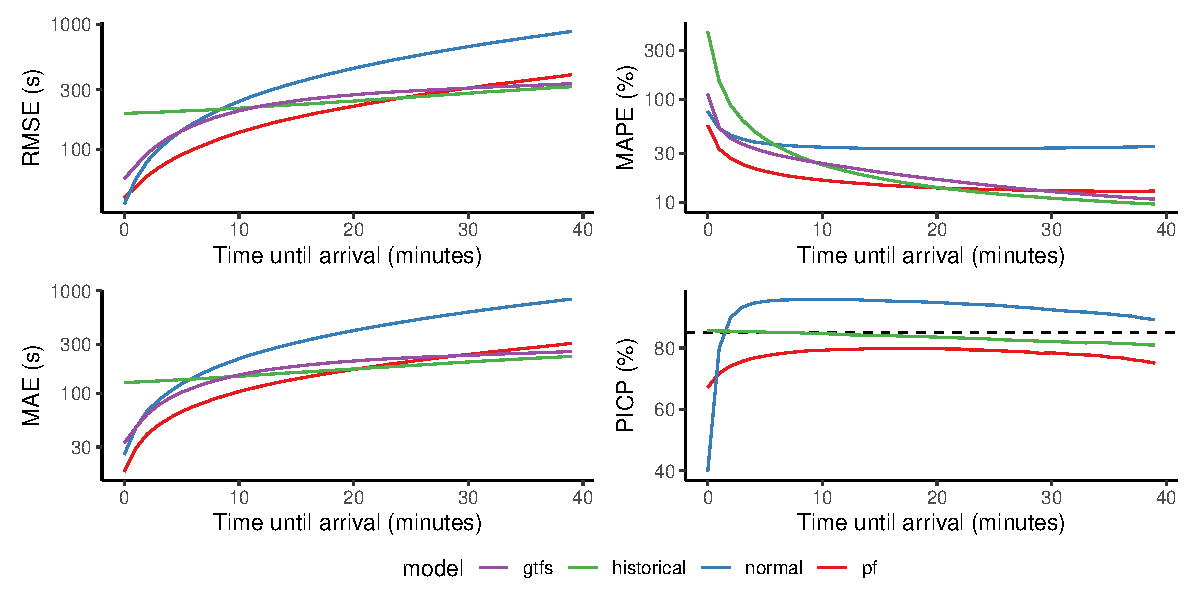
\includegraphics[width=\textwidth]{figure/model_results_rmse_time-1} \caption[Model comparative statistics as a function of time until arrival]{Model comparative statistics as a function of time until arrival. Note the log-scale for RMSE, MAE, and MAPE.}\label{fig:model_results_rmse_time}
\end{figure}


\end{knitrout}


The \gls{rmse} and \gls{mae} for all methods increase with time until arrival as expected, but the rate at which this occurs varies. The three methods that use \rt{} information (\Fpf{}, \Fnorm{}, and \Fsched{}) demonstrate small absolute error when the bus is near, which increases the farther out the bus gets, while \Fhist{} shows a more constant error and far poorer accuracy when the bus is less than 50--10~minutes away. \Fpf{} has the lowest error up until 20~minutes before arrival, and has greater accuracy than \Fsched{} up until 25--30~minutes. This indicates that the current delay is only a useful predictor when the bus has almost arrived, and that accounting for \rt{} traffic conditions \emph{does} improve the accuracy of arrival time prediction. \Fnorm{} quickly shows large prediction errors for all but the nearest buses.




The \gls{mape} for all methods decreases with time until arrival, with \Fhist{} showing the highest relative error when the bus is less than about 5~minutes away. \Fnorm{} remains fairly constant with a large relative error (about 50\%).Again for the first 20~minutes, \Fpf{} has the smallest relative error, and is better than \Fsched{} up until the bus is 25--30~minutes away. After 30~minutes, \Fpf{} seems to converge with slightly lower accuracy than \Fhist{} and \Fsched{}, which appear to be continue improving accuracy after the 40~minute cut-off; however, 89\% of routes in Auckland are less than one hour, so the number of arrival time predictions being made that are greater than 40~minutes becomes small (predictions are only made once the trip starts).


The \gls{picp} is not available for \Fsched{} since that method only provides point estimates. The coverage for the three remaining methods is reasonably constant across time until arrival \cref{fig:model_results_rmse_time}. As we saw earlier, \Fpf{} underestimates uncertainty, resuling in lower than expected coverage, and \Fnorm{} overestimates uncertainty for all times greater than a few minutes. \Fhist{} shows good coverage, although this drops off slightly as time until arrival increases, which could indicate that arrival times for later stops along long routes (since these are the only ones with times until arrival this large) are prone to more variability.




\subsubsection{Stop sequence}

Similarly to time until arrival, we grouped results by stop sequence---skipping the first stop since arrival times are only predicted once the bus begins the trip---and computed the familiar summary statistics, which are displayed in \cref{fig:model_results_rmse_stopn}. Note that stop sequence and time until arrival are correlated, since early stops along a route seldom have long until the bus arrives (once it has begun), and that only 8\% of ~trips have more than 50~stops.


\begin{knitrout}\small
\definecolor{shadecolor}{rgb}{0.969, 0.969, 0.969}\color{fgcolor}\begin{figure}
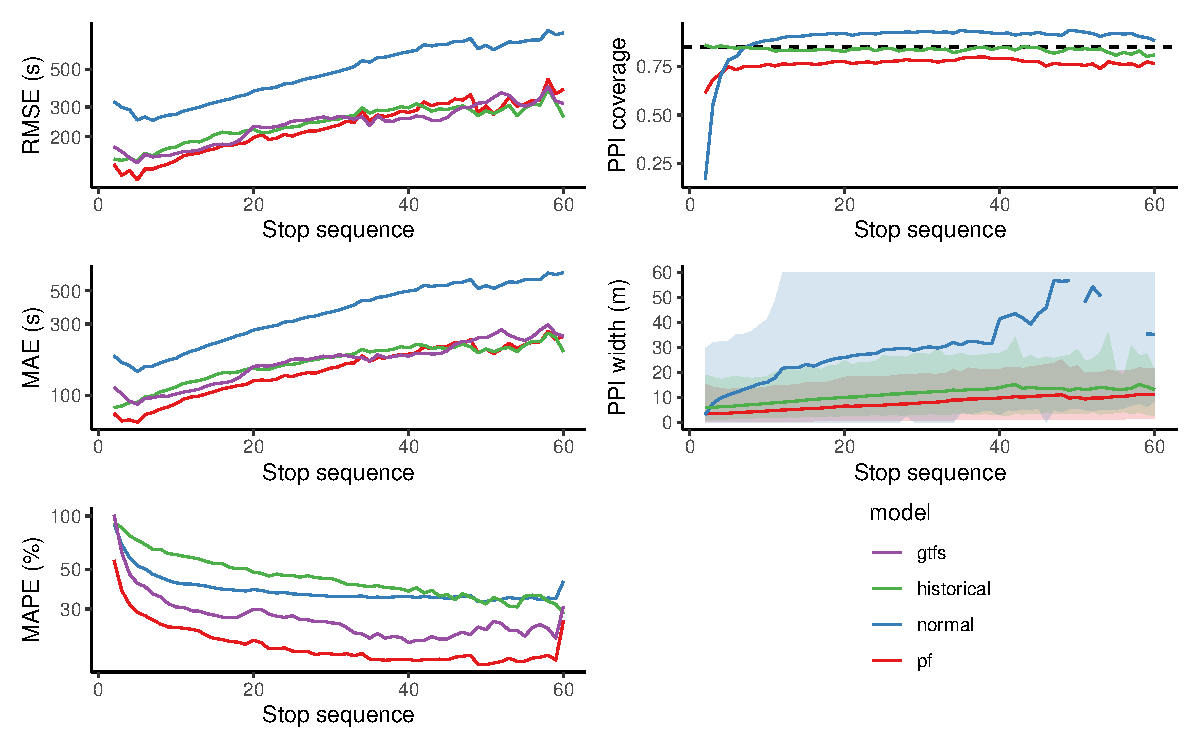
\includegraphics[width=\textwidth]{figure/model_results_rmse_stopn-1} \caption[Model comparative statistics as a function of stop sequence]{Model comparative statistics as a function of stop sequence.}\label{fig:model_results_rmse_stopn}
\end{figure}


\end{knitrout}

The \gls{rmse} and \gls{mae} increase for all models up until stop 50, after which point only few routes have that many stops, so there is increased variability between consecutive stops. As before, \Fnorm{} shows much higher errors than the other three methods, and \Fpf{} shows slightly better prediction accuracy than \Fhist{} and \Fsched{} up until about stop 30, at which point there is no clear difference between these three methods. However, in terms of relative error (\gls{mape}), \Fpf{} outperforms all the others over all stops, while \Fhist{} shows the poorest accuracy particularly for early stops.


The \gls{picp} show much the same trend as before, again not unexpected due to the relationship between stop sequence and time until arrival. \Fpf{} underestimates uncertainty at all stops, while \Fnorm{} overestimates for all but the first few stops---it performs quite poorly for those. \Fhist{} has the desired coverage for all stops.



\subsubsection{Time of day}

We grouped observations into 15~minute intervals over the day and calculated the summary statistics for each prediction method. The results, displayed in \cref{fig:model_results_rmse_timeofday}, differ quite significantly from those seen previously, as we now see a strong peak-hour effect: in the morning there is a single peak (school and work begin at about the same time) at around 8~am, whereas in the evening there are two smaller peaks: one for schools at about 3~pm, and another for workers at around 5~pm.


\begin{knitrout}\small
\definecolor{shadecolor}{rgb}{0.969, 0.969, 0.969}\color{fgcolor}\begin{figure}
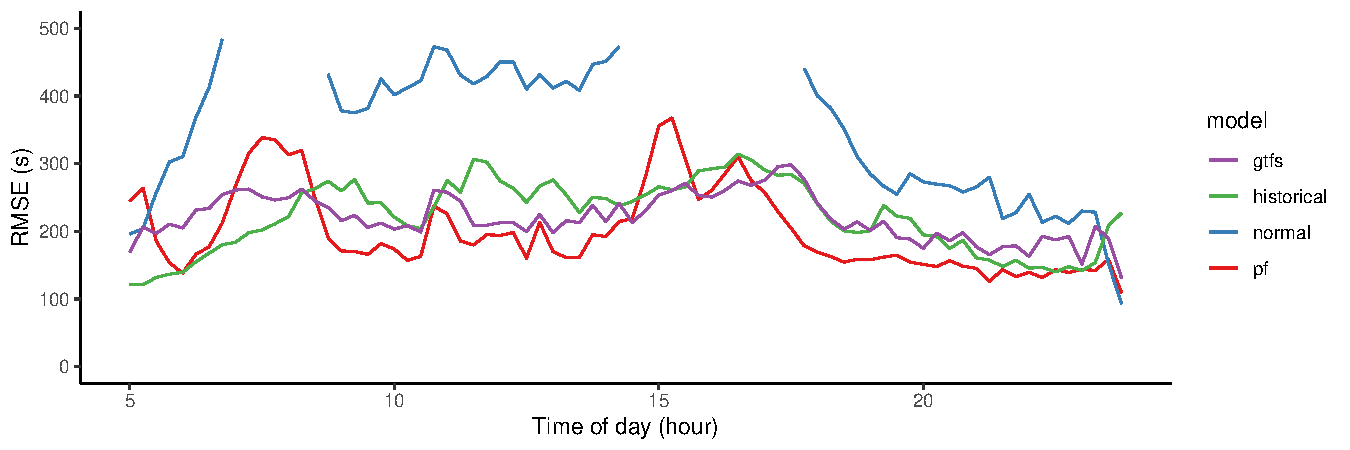
\includegraphics[width=\textwidth]{figure/model_results_rmse_timeofday-1} \caption[Model comparative statistics as a function of time of day]{Model comparative statistics as a function of time of day.}\label{fig:model_results_rmse_timeofday}
\end{figure}


\end{knitrout}

During off-peak (that is, between about 9:30~am and 2:30~pm) \Fpf{} shows the smallest absolute error (\gls{rmse} and \gls{mae}), with \Fhist{} and \Fsched{} showing slightly larger errors. Again, \Fnorm{} shows much poorer accuracy (again, note the log scale). During peak times, all methods show an increase in prediction error as traffic conditions worsen and become more unreliable. \Fsched{} is least affected by this effect since the schedules take, to some extent, peak congestion into account, while the current implementation of our method only uses the \emph{current} traffic state; however, as discussed in \cref{sec:nw_hist_model}, improvements should be possible once a better forecasting method has been implemented.

In terms of relative error (\gls{mape}), we still see the peak effect, but it is much less accentuated, and now \Fpf{} demonstrates the best accuracy throughout the day. This would indicate that much of the absolute error comes from longer-term predictions (when the bus is far away), when traffic has more opportunity to get better or worse: all commuters will be all too familar with how quickly congestion can build. \gls{mape} for \Fsced{} and \Fhist{} show little effect at all of peak hour.


Finally, we look to \gls{picp}, where we can truly see the effect of peak traffic on arrival time predictions, particularly those made using our particle filter. During off-peak, \Fpf{} has very close to the desired coverage of 85\%; during peak time, however, coverage drops quite significantly. This will be due to travel times increasing quickly as congestion builds, meaning initial predictions are too early, and then travel times decreasing again once peak time has passed, and predictions made will be too late. This indicates that, while our \pf{} seems to be able to accurately estimate travel times, it would benefit from the forecasting improvement\footnote{Which we were, unfortunately, unable to complete at this time.}.




\subsection{Assessing the reliability of arrival time prediction}
\label{sec:prediction_model_comp_probs}

\Gls{rmse}, \gls{mae}, and \gls{mape} measure the predictive accuracy of the methods, but do not account for the costs associated with inaccurate predictions. In this section, we evaluate the \emph{reliability} of arrival time distributions by examining
\begin{enumerate}
\item the wait time at the bus stop, and
\item the probability of missing the target bus.
\end{enumerate}
In most cases, the latter incurs a much greater cost, but depends entirely on time until the \emph{next} bus arrival: for high-frequency routes, this will be small; for low-frequency ones, however, it can become quite high\footnote{Some routes only run hourly!}. In this section, we do not differentiate between high and low-frequency routes (we do in \cref{sec:eta_estimates}, however).


The three statistics we compare across the methods are:
\begin{itemize}
\item $\mathbb{P}_m = \Pr{\Varr_m \geq \hat\Tarr_m}$, the probability that the vehicle arrives after the point estimate, $\hat\Tarr_m$, indicating that were a passenger to arrive at the stop by $\hat\Tarr_m$, they would catch the bus with probability $\mathbb{P}_m$;
\item $\mathbb{P}_\ell = \Pr{\Varr_m \geq \hat\alpha_{m,\text{lower}}}$, the probability that the vehicles arrives after the lower bound of the \gls{ppi}; and
\item $\mathbb{E}_\ell = \E{\Varr_m - \hat\alpha_{m,\text{lower}} | \Varr_m \geq \hat\alpha_{m,\text{lower}}}$, the expected waiting time for a passenger arriving at the lower predictive bound, given that the bus arrives after it (that is, conditional on catching the bus).
\end{itemize}


\begin{knitrout}\small
\definecolor{shadecolor}{rgb}{0.969, 0.969, 0.969}\color{fgcolor}\begin{table}

\caption{\label{tab:model_results_pr_miss}The probability of catching a bus given a passenger arrives by the mean/median ($\mathbb{P}_m$) and lower quantile ($\mathbb{P}_\ell$), along with the expected waiting time, in minutes, given arrival by the lower quantile, for each of the for forecast methods.}
\centering
\fontsize{8}{10}\selectfont
\begin{tabular}[t]{lrrrl}
\toprule
  & $\mathbb{P}_m$ (\%) & $\mathbb{P}_\ell$ (\%) & $\mathbb{E}_\ell$ (m) & 5--90\% CI\\
\midrule
\Fpf{}: Particle filter & 64 & 93 & 4.4 & 0.3--10.2\\
\Fnorm{}: Normal approximation & 96 & 98 & 20.9 & 2.9--37.6\\
\Fhist{}: Historical delays & 54 & 98 & 7.1 & 1.1--14.1\\
\Fsched{}: Schedule-delay & 38 &  &  & \\
\bottomrule
\end{tabular}
\end{table}


\end{knitrout}



The overall results are displayed in \cref{tab:model_results_pr_miss}. If a passenger, at any time, looks at the \gls{eta} of their bus \emph{once} and arrives at the stop by the indicated time, then using \Fpf{} their probability of catching the bus is almost double that of using \Fsched{}. Using \Fhist{}, then (not surprisingly) $\mathbb{P}_m$ is about 50\%; \Fnorm{} is over 95\% which indicates that it is underestimating arrival times.



The concept behind examining the accuracy of the lower quantile, $\mathbb{P}_\ell$, is that this value should give passengers the best chance of catching the bus. We used the 2.5\% quantile for the lower estimate, so we would expect the bus to arrive after the predicted time 97.5\% of the time. This is the case for \Fnorm{} and \Fhist{}, but \Fpf{} has a slightly lower probability that expected. Associated with the lower bound is the expected wait time until the bus actually arrives, conditional on not having missed it ($\mathbb{E}_\ell$). \Fpf{} has the shortest expected wait followed closly by \Fhist{}, while the wait time using \Fnorm{} is about four times as long as with \Fpf{}.



Since \Fsched{} provides only a point estimate, we cannot compare it directly to the other methods, in particular \Fpf{}. To do so, we can \emph{indirectly} compare these methods by proposing a passenger arrives $x$~minutes before the stated arrival time (by \Fsched{}) and calculating the probability of capture and expected wait time. The resulting curves are shown for a range of times (arriving 4--12~minutes before the stated arrival) in \cref{fig:model_results_pr_gtfs}, with the values for the other three methods overlaid with dashed lines.



\begin{knitrout}\small
\definecolor{shadecolor}{rgb}{0.969, 0.969, 0.969}\color{fgcolor}\begin{figure}

{\centering 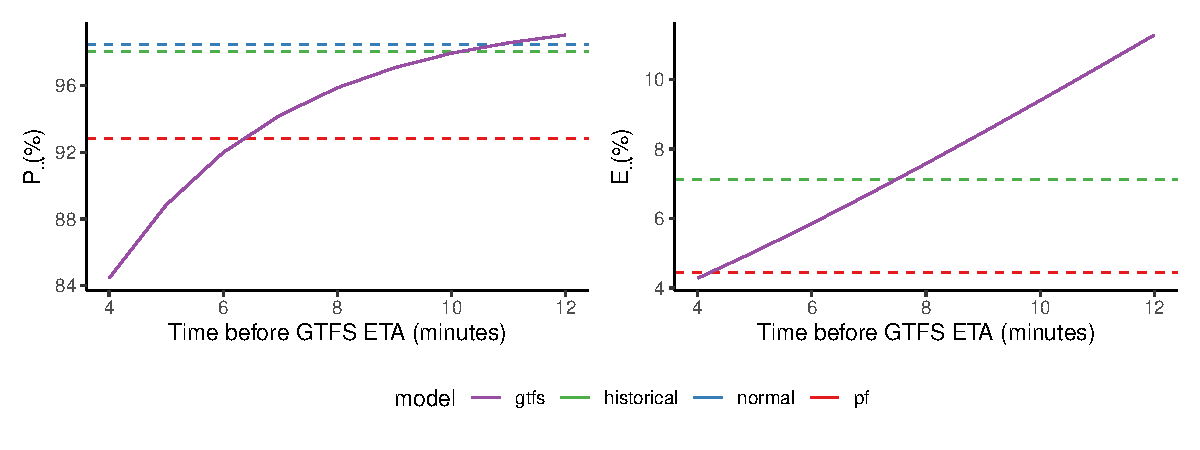
\includegraphics[width=\textwidth]{figure/model_results_pr_gtfs-1} 

}

\caption[GTFS equivalent]{GTFS equivalent}\label{fig:model_results_pr_gtfs}
\end{figure}


\end{knitrout}



First let us consider the probability of the bus arriving after the estimated arrival time, $\mathbb{P}_\ell$. Based on the data collected, a passenger would need to arrive at least 10~minutes before the stated \gls{eta} (by \Fsched{}) to have a 97.5\% probability of catching the bus. To obtain the same probability as \Fpf{}, this would be 6~minutes before arrival. Now we can compare the expected waiting time: to achieve the targetted 97.5\% chance of catching the bus, the passenger would arrive 10 minutes before the stated \gls{eta}, which has an expected waiting time of about 9~minutes. Or, arriving 6~minutes before, the expected wait time drops to almost 6~minutes, which is greater than the expected wait time under \Fpf{} of just over 4~minutes.


We could also examine this the opposite way, and match the expected waiting time with that of \Fpf{}. In this case, a passenger would need to arrive no more than 4~minutes before the stated arrival time, which would give them an 85\% chance of catching the bus. For the remainder of this section, we use 6~minutes before the specified \gls{eta} to obtain a lower bound for \Fsched{}, and compare the probabilities as a function of time until arrival, stop sequence, and time of day.



\subsubsection{Time until arrival}

\Cref{fig:model_results_pr_time} shows $\mathbb{P}_m$, $\mathbb{P}_\ell$, and $\mathbb{E}_\ell$ computed for one-minute intervals for each of the four methods. For \Fsched{}, we used a lower bound of 6~minutes before the predicted arrival. For the expected wait time, we also computed the 5\% and 90\% quantiles, which are displayed as shaded regions. The dotted line in the expected waiting time graph represents the maximum possible waiting time; that is, when the bus is 10~minutes and you arrive immediately at the stop, you will wait 10~minutes.


\begin{knitrout}\small
\definecolor{shadecolor}{rgb}{0.969, 0.969, 0.969}\color{fgcolor}\begin{figure}
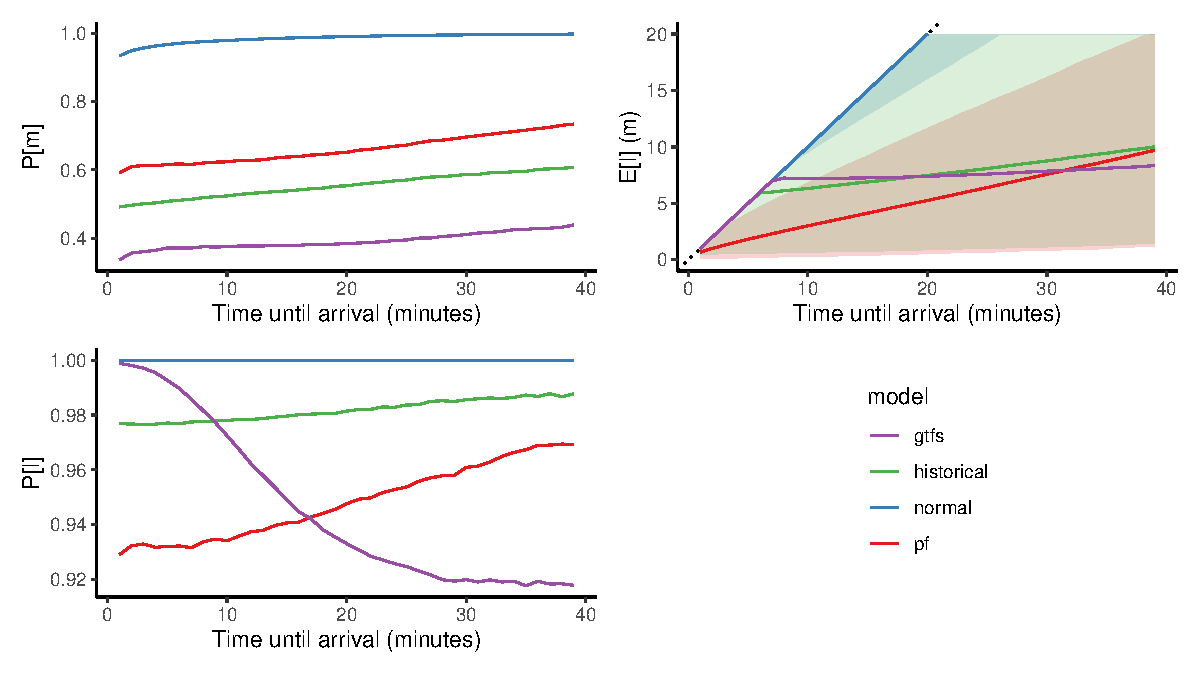
\includegraphics[width=\textwidth]{figure/model_results_pr_time-1} \caption[Summary values by time until arrival]{Summary values by time until arrival.}\label{fig:model_results_pr_time}
\end{figure}


\end{knitrout}



The probability that the bus arrives after the point estimate (mean or median), $\mathbb{P}_\ell$ is more or less constant with a slight decrease as the bus nears the stop. \Fpf{} and \Fnorm{} are above the expected value of 50\%, though the latter is significantly higher. \Fnorm{} performs reasonably well, though tends to underestimate arrival time the farther out the bus is, while \Fsched{} overestimates arrival time quite such that there is less than a 40\% chance of catching the bus if it is less than 20~minutes away.


As for $\mathbb{P}_\ell$, we see a different trend: \Fpf{} and \Fhist{} increase the further out the vehicle is; on the other hand with \Fsched{}, the probability decreases, although this is because we have chosen a fixed lower bound. Once the bus is about 15~minutes away, the \gls{eta} provided by \Fsched{} minus 6~minutes is increasingly likely to result in a caught bus, while under \Fpf{} this probability is lower, indicating not enough uncertainty is accounted for over short distances (though the difference is only a few percent).


Finally, we look at the expected waiting time, given a passenger arrives at the lower bound \emph{and} the bus arrives after it. \Fpf{} has a consistently shorter waiting time, though by about 30~minutes out the three methods (excluding \Fnorm{}) are approximately the same. We can see that the expected waiting time for \Fsched{} is more or less independent of time until arrival, which is to be expected since the width is fixed. The shaded reasons represent the 5\% and 90\% quantiles of waiting time, and we see that \Fpf{} results in shorter waits, on average, for 10~minutes before arrival. As for the normal approximation, it tends towards overestimation of arrival time uncertainty, so expected waiting time is very large if arriving at the lower estimate, indicating that \Fnorm{} is not a reliable choice of predictor.



\subsubsection{Stop sequence}

The same values were computed by stop sequence, and displayed in \cref{fig:model_results_pr_stop}. Again, \Fhist{} achieves the target probability of 50\%, whilc \Fpf{} is slightly above at about 60\%. Most notable is the steady decline in the reliability of \Fsched{}, which after stop 40 drops to about a one in three chance of catching the bus (assuming you arrive at the predicted \gls{eta}).



\begin{knitrout}\small
\definecolor{shadecolor}{rgb}{0.969, 0.969, 0.969}\color{fgcolor}\begin{figure}
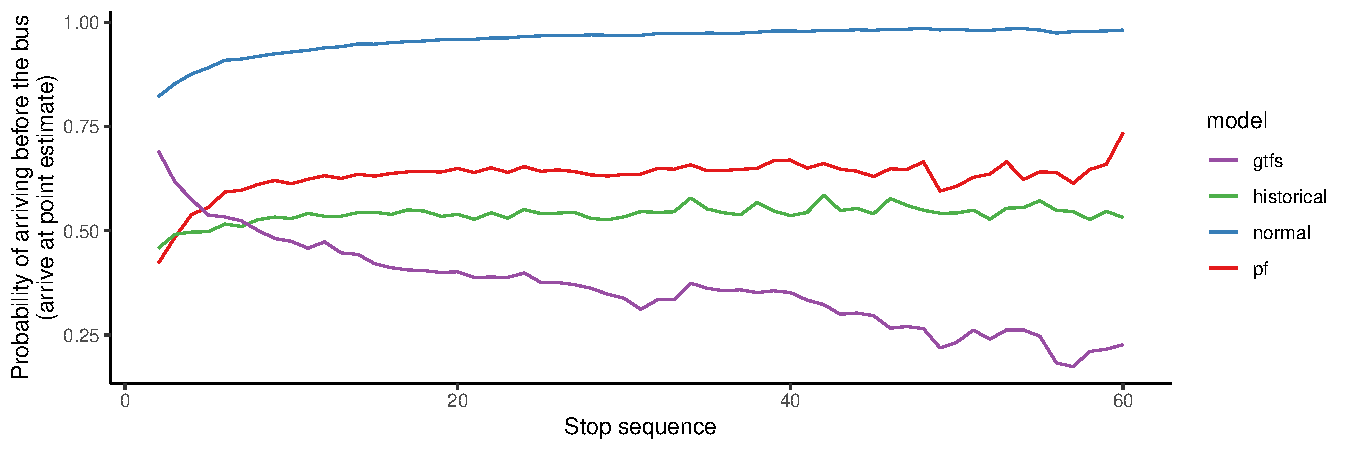
\includegraphics[width=\textwidth]{figure/model_results_pr_stop-1} \caption[Summary values by stop sequence]{Summary values by stop sequence.}\label{fig:model_results_pr_stop}
\end{figure}


\end{knitrout}


Moving on to the lower 2.5\% quantile, $\mathbb{P}_\ell$, we expect 97.5\% probabiltiy of capture. We see that, as before, \Fpf{} overestimates arrival time slightly, at about 90\%, while \Fsched{} decreases (again) with stop sequence; but remember the lower bound was fixed at 6~minutes before the predicted \gls{eta}. The associated wait time, $\mathbb{E}_\ell$, increases for all methods with increasing stop sequence \emph{except} for \Fsched{}, which decreases (again, the width is fixed). \Fpf{} has the lowest expected wait time up until about stop 50, and again the upper 90\% interval is lower than the mean for \Fsched{} for the first 20~stops. However, many stops with low indices will be serviced within the first 5--10~minutes of the trip, thus inflating $\mathbb{P}_\ell$ under \Fsched{}.



\subsubsection{Time of day}

The probabilities and expected waiting time were calculated for 15~minute intervals over the day for each of the models, as is shown in \cref{fig:model_results_pr_timeofday}. The peak hour effects are again visible, associated with an increased probability of arriving before the bus does under \Fpf{} for both the median and lower 2.5\% quantile, while for \Fsched{} the probability of arriving before the bus does decreases slightly. In the evening we see the performance of \Fpf{} drops rapidly, which likely indicates that the probability of stopping is much reduced (many evening services have low occupancy, and as such are less likely to stop at each stop). Future work targetting more complicated dwell time models could help to correct this, however.


\begin{knitrout}\small
\definecolor{shadecolor}{rgb}{0.969, 0.969, 0.969}\color{fgcolor}\begin{figure}
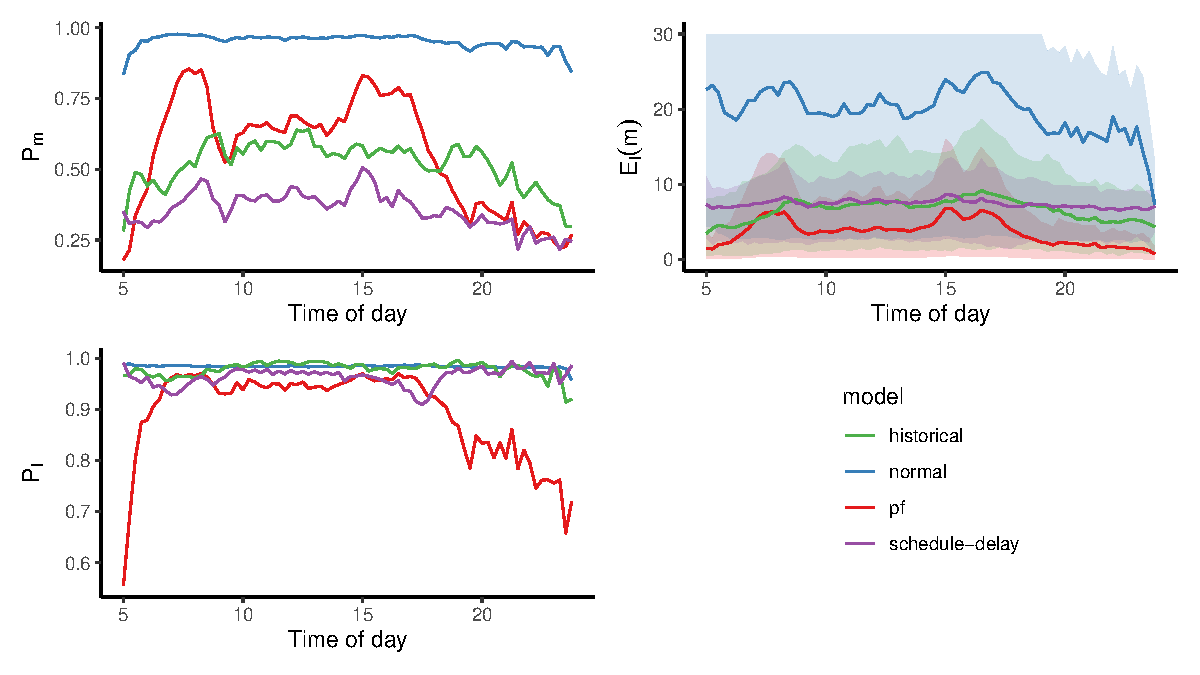
\includegraphics[width=\textwidth]{figure/model_results_pr_timeofday-1} \caption[Summary values by time of day]{Summary values by time of day.}\label{fig:model_results_pr_timeofday}
\end{figure}


\end{knitrout}


We see much the same pattern with the expected waiting time $\mathbb{E}_\ell$, in which wait times increase by a few minutes under \Fpf{}, while there is little noticable change for \Fsched{} and \Fhist{}. Even so, \Fpf{} consistently provides shorter expected wait times than \Fsched{}, and over most of the day (from about 7~am until 6~pm) the probability of the bus arriving after the lower estimate is above 90\%.
]


\subsection{Result summary}
\label{sec:prediction_model_comp_summary}


The results in \cref{sec:prediction_model_comp_stats,sec:prediction_model_comp_probs} demonstrate the relative accuracy and reliability of four methods of predicting the arrival time distribution at a stop. The particle filter (\Fpf{}) uses a sample of weighted particles representing the vehicle's state, along with the \rt{} traffic state, to approximate the distribution. On average, it is slightly more accurate that the currently used method (\Fsched{}), particularly when the bus is within 20~minutes of arriving and during the daytime off-peak period, and covers most of the uncertainty during this period (as per \gls{picp}).

As for the reliability of the estimates---that is, their use as an \gls{eta} for commuters---the \pf{} tended to underestimate the median arrival time, whereas the current method tends to \emph{overestimate} the point estimate; in terms of the application, the former is prefered, often resulting in a 30\% higher probability of catching the bus (that is, not missing it). The \pf{} provides an estimate of the arrival time distribution, allowing us to estimate quantiles easily\footnote{Except for the computational burden.}. We showed that the lower bound typically was an overestimate, indicating that perhaps not enough variability was being included, or perhaps that more particles are needed; we used $\tilde N = 200$, but future work could involve modifying this depending on the number of stops remaining along a route. However, the lower bound still gives a 90--95\% chance of catching the bus in most cases, and has a significantly shorter wait compared to the current method (assuming one arrives 6~minutes before the specified time). This indicates that the \pf{}, as well as providing improved prediction accuracy, can also provide more reliability for passengers.


In the results we saw that there were a few scenarios that could be attributed to much of the \pf{}'s poorer performance: peak times and evenings. Further work could be performed, particularly on forecasting network travel times, to improve these predictions. We also presented two other models: a normal approximation (\Fnorm{}), which demonstrated very poor performance in that it tended to overestimate the distribution uncertainty, likely a result of combining the mixtures; historical data (\Fhist{}) was also used---the arrival time prediction distribution was based purely on the distribution of arrival time delays at stops along a route---which performed admirably, with good estimation of the distribution quantiles, but as would be expected did not perform once the trip was underway and \rt{} information was available. It does, however, suggest that this historical data should (and will be) used for prior predictions of arrival time; that is, before a trip has registered with the \rt{} service, the best prediction of arrival time will be using \Fhist{}.
